\chapter{Related Work}
\label{chap:relwork}

The area of relational learning in the context of Semantic Web has recently attracted interest from many researchers. The approaches that aim at tackling this problem can be mainly classified into three groups: statistics-based, text-based and logic-based. In this chapter we review Semantic Web and the relevant works from these groups.

\section{Semantic Web}

The Semantic Web~\cite{ref26} enables computers to interpret the meaning of the data all over the Internet. Alternatively, it is defined as ``a web of data that can be processed directly and indirectly by machines".

The World Wide Web Consortium (W3C) defines the Semantic Web and the Resource Description Framework (RDF) as a platform for Linked Data~\cite{ref26}. The W3C proposes other technologies such as SPARQL and OWL for data manipulation. Architecture of the W3C is presented as a stack in Figure~\ref{fig1}~\footnote{\url{https://www.w3.org/DesignIssues/diagrams/sweb-stack/2006a.png}}.

\begin{figure}
\centering
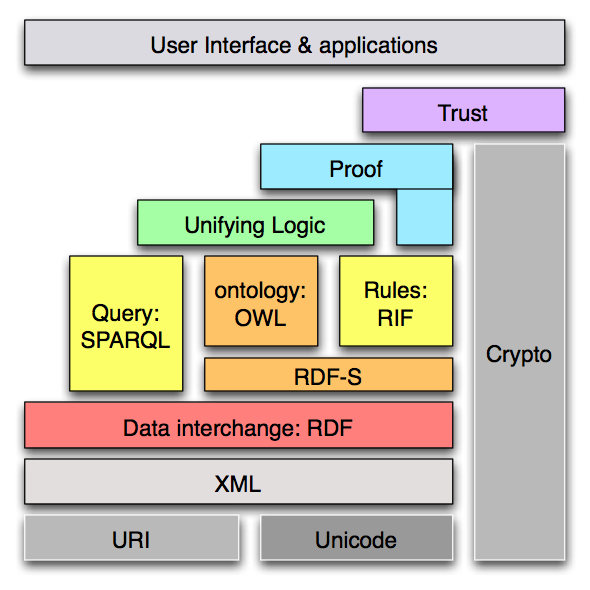
\includegraphics[width=0.65\textwidth]{figures/semantic_web.png}
\caption{The Semantic Web technologies}
\label{fig1}
\end{figure}

The RDF is widely used for representing KGs and this is the fundamental format for many KGs such as YAGO~\cite{ref28}, FreeBase~\footnote{\url{https://developers.google.com/freebase/}}, Wikidata\footnote{\url{https://www.wikidata.org}}, etc. There are several prominent examples of KGs and their sizes in Table~\ref{table1}~\cite{ref27}. Google's Knowledge Graph is the largest among all the KGs mentioned in the table with 18 billions facts. In our current work, we focus on YAGO, IMDB for experimental results because our theory framework can be tested on different scales.

Though having different number of predicates, entities and facts, these graphs share the following common properties~\cite{ref27}:

\begin{itemize}
\item KGs reflect facts from real world.
\item KGs cover different domains, for example, general purpose in YAGO or domain specific such as movie in IMDB.
\item The interconnection between knowledge graphs are taken into consideration, i.e., the mapping of entities and relations are explicitly indicated in each KG.
\end{itemize}

\begin{table}
\begin{center}
\begin{tabular}{|c|c|c|c|c|}
\hline
Name & Instances & Facts & Types & Relations\\
\hline\hline
DBpedia (English) & 4,806,150 & 176,043,129 & 735 & 2,813\\
\hline
YAGO & 4,595,906 & 25,946,870 & 488,469 & 77\\
\hline
Freebase & 49,947,845 & 3,041,722,635 & 26,507 & 37,781\\
\hline
Wikidata & 15,602,060 & 65,993,797 & 23,157 & 1,673\\
\hline
NELL & 2,006,896 & 432,845 & 285 & 425\\
\hline
OpenCyc & 118,499 & 2,413,894 & 45,153 & 18,526\\
\hline
Google's Knowledge Graph & 570,000,000 & 18,000,000,000 & 1,500 & 35,000\\
\hline
Google's Knowledge Vault & 45,000,000 & 271,000,000 & 1,100 & 4,469\\
\hline
Yahoo! Knowledge Graph & 3,443,743 & 1,391,054,990 & 250 & 800\\
\hline
IMDB & 117,551 & 134,639 & 17,049 & 39 \\
\hline
\end{tabular}
\end{center}
\caption{List of typical knowledge graphs}
\label{table1}
\end{table}

\section{Statistics-based Approaches for Relational Learning}

Relational learning is a research that ``represent, reason and learn in domains with complex relational structure"~\cite{ref43}. Many frameworks in this field are fundamentally suitable for Semantic Web, and thus, both research aspects develop hand-in-hand together. In this section, we discuss about relational learning from statistics view. The statistics-based approaches focus on building models with latent features which are not directly observable from the original data~\cite{ref1}. The core idea is to infer correlation between objects based on selected hidden features. Besides, feature extraction is automatically executed in these methods.

RESCAL is one of principal algorithms in this direction where relations of all hidden feature pairs are taken into consideration~\cite{ref2, ref3}. This method is extended to classical tensor decomposition algorithm~\cite{ref4} and neural tensor network~\cite{ref5}.

While many tensor factorization methods use subject, predicate and object as three dimensions to model a knowledge graph as a cube, some matrix decomposition algorithms try to transform this cube into a two dimensional data. For instance, in~\cite{ref6, ref7} subject and object dimensions are merged into one representing a pair of entities.

Distance-based models use the intuition that entities have high chance to be related to each other if their hidden representation features are close to each other. The closeness can be checked based on some predefined distance measures. This approach can be expanded to structure embedding model~\cite{ref8}.

\section{Logic-based Approaches for Relational Learning}

The logic-based approaches aim at finding observable patterns in order to infer new links in the knowledge graph~\cite{ref1}. Since the patterns can be directly seen in the data, these algorithms are more interpretable than the ones based on statistical approaches. For instance, a pattern extracted from the graph in Figure~\ref{fig1.1} can be represented as rule $r1$ in Section~\ref{chap:motivation}. This rule reflects a triangular pattern in the KG, where the edges of the triangle are labeled with the predicates appearing in the rule. Since this pattern is frequently observed, it can be mined in order to predict new links in the KG. For instance, if we apply rule $r1$ to a KG in the Figure~\ref{fig1.1}, we can deduce the fact \textit{livesIn(Lucy, Amsterdam)}.

In the rest of this section, we review some of the most prominent logic-based relational learning systems in details and illustrate with typical examples.

\subsection{Inductive Logic Programming Systems}

Inductive Logic Programming~\cite{ref9} (ILP) is a combination of Machine Learning and Logic Programming fields and it is used for generating hypothesis based on background knowledge and specific examples. These examples can be classified into positive and negative ones. The goal is to find a hypothesis that covers all positive examples and none of the negative ones.

Rule mining is a core problem in ILP, however, applying ILP algorithms to semantic web data is problematic for the following reasons. First, ILP tools are not scalable for large knowlege graphs such as YAGO, Freebase, Wikidata~\cite{ref10}. In some experiments conducted in~\cite{ref10}, it has been shown that the cutting edge ILP tools, for example, ALEPH~\cite{ref14, ref10}, QuickFoil~\cite{ref15, ref10} require several days to process YAGO2.

Second, ILP methods use closed world assumption (CWA), under which a given KG is assumed to be complete and missing facts are treated as false rather than unknown. ILP methods require both positive and negative examples, which are similar to traditional machine learning algorithms. CWA is not suitable for our problem since in the KGs the positive examples are incomplete and negative ones are unknown~\cite{ref10}.

Third, most ILP algorithms generate positive Horn rules without exceptions~\cite{ref11}. Since these rules may have low precision, exceptions should be taken into consideration to improve the quality of facts the rules predict. Therefore, mining exceptions from rules is an important purpose of our work and naively using ILP techniques is not always possible in our setting. In the following paragraphs, some popular ILP systems are described in details.

\textbf{ALEPH.} This name stands for A Learning Engine for Proposing Hypotheses which is one of the typical systems in ILP. This tool is developed and extended from P-Progol~\footnote{\url{http://www.cs.ox.ac.uk/activities/machinelearning/Aleph/aleph}}. Like many other ILP systems, as input ALEPH receives the background knowledge and sets of positive, negative examples. After that, it generates a set of rules as a hypothesis set. More specifically, the tool processes data in the following steps:

\begin{itemize}
\item ALEPH picks an example to hypothesize and terminates if there is not any.
\item The most specific rule that infers the example is found.
\item Among all subsets, that is, combinations of atoms in the most specific rule, the chosen one with the highest score is added to the hypothesis set.
\item All examples inferred by the chosen one are removed from the data and ALEPH comes back to the first step.
\end{itemize}

Though this method is one of the most popular tools in ILP, experiments in~\cite{ref10} show that its run time can be up to days. This indicates that ALEPH is not scalable for large datasets.

\textbf{QuickFOIL.} To address the scalability issues of ILP systems, the system QuickFOIL which is an optimized version of FOIL~\cite{ref36} has been developed. In each stage QuickFOIL produces a new Horn rule that optimizes some measure score. Whenever this rule covers an example, the latter is removed from the set of positive ones. Intuitively, the collection of found rules in each step can be used to summarize original dataset. QuickFOIL uses data refinement and pruning techniques to process large-scale input with millions of facts. This tool is a traditional ILP system since it requires negative examples and uses CWA assumption.

\subsection{Relational Learning Systems}

Relational Learning systems do not require negative examples in the data, thus, also work well under the Open World Assumption (OWA) and this makes them attractive for our setting. In addition, with the aim to expand KG, new facts generated by applying rules as an output of Relational Learning to the original KG are more precise than those of traditional Information Extraction~\cite{ref29}. Indeed, relational learning methods have been successfully applied to predict facts in YAGO2~\cite{ref30}.

\textbf{WARMR.} The WARMR~\cite{ref16, ref17} system represents a combination of traditional ILP and relational learning approaches. The core idea is that infrequent queries are not necessary to be expanded by adding an atom, because this operation results in new infrequent ones again~\cite{ref17}. WARMR exploits this pruning technique in level-wise search to mine patterns. More specifically, at each level, infrequent queries are removed and the remaining frequent ones are expanded using the above operation. New queries are deleted if they can be expanded from an infrequent one in previous level. This step is repeated until we cannot generate new queries. This idea is similar to APRIORI algorithm~\cite{ref44} in exploratory data mining. To check the runtime performance of WARMR, AMIE+ authors~\cite{ref10} test it on the YAGO2 dataset. The tool processes more than a day with YAGO2. In general, WARMR is developed with ProLog, and thus, is not fast to process big data~\cite{ref10}.

\textbf{AMIE(+).} The scalability and CWA assumption issues of ILP are tackled in AMIE(+)~\cite{ref10} system. This tool receives a large knowledge graph as an input and generates top positive Horn rules of high quality. Initially, AMIE begins with a list of rules with empty body and binary head predicate. After that, the rules can be expanded with additional relations and variables by three mining operators. These operators are executed by query manipulation to explore new predicates and instances. As regards the implementation, AMIE uses in-memory database with fact indexes to run select and existence queries.

AMIE+ is a new version of AMIE whose run time performance is enhanced by exploiting rule optimization and confidence assessment. With rule optimization, the authors introduce three pruning strategies: maximum length constraint, quality condition and simplifying query. More specifically, in the first two strategies, a rule is not expanded if its length reaches a threshold or it is perfect. As regards confidence assessment, approximation techniques are conducted to improve the runtime. Experimental work in~\cite{ref10} shows that this platform can process millions of triples in RDF graph and it surpasses other methods in terms of run time efficiency.

\textbf{RDF2Rules.} The RDF2Rules~\cite{ref29} focuses on mining cyclic patterns from KGs, which are postprocessed and cast into rules. Besides, this tool exploits entity types to create and test mined rules. As a result, the rule quality is enhanced and the authors use a new confidence measure to verify this. Experiments show that this tool is efficient, especially with rules containing entity type, it run much faster than AMIE+. However, the form of the mined rule is restricted to cycles, which makes the system more restrictive than the AMIE+.

Like other ILP platforms, Relational Learning tools do not learn nonmonotonic rules, that is, rules with exceptions; they only focus on positive (Horn) rules. In our work, we aim at bridging this gap and also learn the latter types of rules.

\subsection{Nonmonotonic Rule Mining Systems}
\label{related-work-nonmonotonic-rule-mining-systems}

Rules with exceptions are traditionally learned by nonmonotonic rule learning systems. As regards a relation between ILP and Abductive Logic Programming (ALP~\cite{ref31}), a research work in~\cite{ref32} is conducted to find rules with exceptions. Its core idea is to convert an ILP problem to an ALP one, thus, ALP methods can be exploited to find outputs of ILP. However, this system adopts CWA, and therefore cannot be applied in our work. There is another nonmonotonic rule learning method that accounts for incomplete data~\cite{ref34} where a coordination of Semantic Web ontology and positive/negative rules is exploited to explore patterns. This work pays attention to complicated communication between different reasoning components. This is different from the current work where we focus on the quality of the predicted data. By contrast, the setting of the following research is close to that of the thesis.

\textbf{Nonmonotonic Rule Mining under OWA over the flattened data.} The work made some steps towards learning nonmonotonic programs from incomplete KGs~\cite{ref12}. This tool works on the flattened KG, that is, the graph in which all RDF triples are converted to unary facts by concatenating predicates and objects. More specifically, a binary fact such as \textit{bornIn(s1, US)} is transformed to a fact in the unary form \textit{bornInUS(s1)}. This way, a KG is converted to a binary transaction table (see Table~\ref{table2} as an example) where elements 1 or 0 mean the facts generated by corresponding rows and columns appear in the original graph or not, respectively. For instance, from Table~\ref{table2} we can see that \textit{bornInUS(s1)} is included in the KG but \textit{livesInUS(s6)} is not. This representation allows one to apply highly optimized Item Set Mining algorithms~\cite{ref37} to extract data patterns. These patterns are then used to create positive association rules~\cite{ref13}.

\begin{table}
\begin{center}
\begin{tabular}{|c|c|c|c|c|}
\hline
 & bornInUS & livesInUS & immigratesToUS & livesInUK\\
\hline\hline
s1 & 1 & 1 & 0 & 0\\
\hline
s2 & 1 & 0 & 1 & 1\\
\hline
s3 & 1 & 1 & 0 & 1\\
\hline
s4 & 0 & 0 & 1 & 0\\
\hline
s5 & 1 & 0 & 0 & 1\\
\hline
s6 & 0 & 0 & 1 & 1\\
\hline
s7 & 0 & 0 & 1 & 1\\
\hline
s8 & 1 & 0 & 0 & 0\\
\hline
s9 & 1 & 1 & 1 & 1\\
\hline
s10 & 0 & 1 & 0 & 1\\
\hline
\end{tabular}
\end{center}
\caption{Transaction table as flattened knowledge graph data.}
\label{table2}
\end{table}

In the next step, the exceptions for each rule are found and ranked based on several score measures and innovative concept of Partial Materialization (PM)~\cite{ref12}. The core idea of PM is that the authors want to enable the interaction between revised rules. A difference between the thesis and~\cite{ref12} is the format of the data. While in~\cite{ref12} binary facts are translated to unary ones, in this thesis we keep the facts in their natural relational format.

\section{Text-based Approaches}

Both of statistics-based and logic-based approaches are internal methods, that is, only data inside the graph is used to infer new relations. On the contrary, this section focuses on different approaches that require data outside the KG, that is, web pages linking to objects or big collection of documents.

Wikipedia pages can be used to identify relations between entities~\cite{ref18}. On a larger scale, an algorithm in~\cite{ref19} is developed to learn lexical predicate patterns, for example, \textit{isMarriedTo} predicate in Figure~\ref{fig1.1} can be expressed  as ``married to", ``engaged with", etc in some documents. Then these patterns are searched all over the Internet to find subject-object pairs corresponding to them. These new pairs can be added to the original graph. As a result, a big text corpora is used in ~\cite{ref19} to learn relations.

Assuming that entities appearing in the same table should have the same relations, authors in~\cite{ref20} try to refine KG based on Wikipedia tables. Similarly, ~\cite{ref21}, ~\cite{ref22} exploit page lists or HTML tables, respectively.

Instead of documents, interlinks between the same entities in different KGs are used to add new facts~\cite{ref23, ref24}. More specifically, relations of two entities in FreeBase can be inserted into YAGO if they also appear in the latter knowledge graph. In~\cite{ref25} this approach has been extended to a probabilistic setting, where for every deduced relation a corresponding probabilistic weight is computed.